% Created 2016-03-05 Sat 15:47
\documentclass[bigger]{beamer}
\usepackage[utf8]{inputenc}
\usepackage[T1]{fontenc}
\usepackage{fixltx2e}
\usepackage{graphicx}
\usepackage{grffile}
\usepackage{longtable}
\usepackage{wrapfig}
\usepackage{rotating}
\usepackage[normalem]{ulem}
\usepackage{amsmath}
\usepackage{textcomp}
\usepackage{amssymb}
\usepackage{capt-of}
\usepackage{hyperref}
\usetheme{CambridgeUS}
\AtBeginSection{\begin{frame}{Outline}   \tableofcontents[currentsection] \end{frame} }
\setbeamertemplate{navigation symbols}{}
\renewcommand\maketitle{\frame[plain]{\titlepage}}
\usepackage{fontspec}
\usepackage{xeCJK}
\setmainfont{Times New Roman}
\setsansfont{Arial}
\setmonofont{Courier Std}
\setCJKmainfont[BoldFont={ },ItalicFont={ }]{WenQuanYi Micro Hei}
\setCJKsansfont{WenQuanYi Micro Hei}
\setCJKmonofont{WenQuanYi Micro Hei Mono}
\graphicspath{{pic/}}
\usepackage[backend = biber, natbib=true, style = science, sorting = none]{biblatex}
\addbibresource{Pharmaron.bib}
\AtBeginBibliography{\footnotesize}
\setbeamertemplate{bibliography item}[text]
\usepackage[none]{hyphenat}
\usepackage[abs]{overpic}
\usetheme{default}
\author{Xiaowei Mao}
\date{\today}
\title{Multiple therapeutic effects of progranulin on experimental acute ischaemic stroke}
\date[March 4$^{th}$, 2016]{March 4$^{th}$, 2016 \\ \vskip 0.5cm \scriptsize{Brain. 2015 Jul;138(Pt 7):1932-48.}}
\title[Progranulin on ischemic stroke]{Multiple therapeutic effects of progranulin on experimental acute ischaemic stroke}
\institute[Pharmaron]{Pharmacology, Pharmaron}
%\logo{
\includegraphics[height=5mm]{logo.png}}
\hypersetup{
 pdfauthor={Xiaowei Mao},
 pdftitle={Multiple therapeutic effects of progranulin on experimental acute ischaemic stroke},
 pdfkeywords={},
 pdfsubject={},
 pdfcreator={Emacs 24.5.1 (Org mode 8.3.4)}, 
 pdflang={English}}
\begin{document}

\maketitle
\begin{frame}{Outline}
\setcounter{tocdepth}{1}
\tableofcontents
\end{frame}

\section{Background}
\label{sec:orgheadline10}
\begin{frame}[label={sec:orgheadline1}]{What's the stroke}
\begin{columns}
\begin{column}{0.6\columnwidth}
\begin{itemize}
\item A stroke is a medical emergency in which the blood supply to any portion of the brain is interrupted or reduced.
\end{itemize}
\vspace{0.5cm}
\begin{itemize}
\item Alternative names: Cerebrovascular accident/ disease (CVA), Cerebral infarction, Cerebral hemorrhage.
\end{itemize}
\end{column}
\begin{column}{0.4\columnwidth}
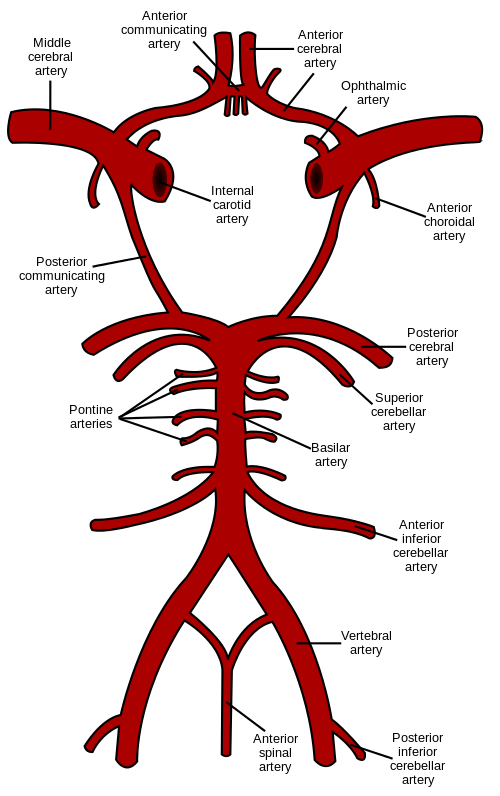
\includegraphics[width=4.5cm]{b1} \newline
\centering \scriptsize{The Circle of Willis Anatomy}
\end{column}
\end{columns}
\end{frame}
\begin{frame}[label={sec:orgheadline2}]{What's the impact of stroke?}
\begin{itemize}
\item Stroke is the third leading cause of death in the United States (First in China)
\begin{itemize}
\item Someone suffers a stroke every 40 seconds
\item About 795,000 Americans suffer a stroke each year (2\% in 2012-2013)
\item About every 4 minutes, someone dies of a stroke
\end{itemize}
\item Stroke is a leading cause of serious, long-term long disability
\item About 6.4 million Americans are stroke survivors
\item Americans will pay about \$71.5 billion in 2012 for stroke-related related medical costs and lost productivity (¥40 billion in China)
\end{itemize}
\end{frame}
\begin{frame}[label={sec:orgheadline3}]{Types of stroke}
\begin{overpic}[height=6cm, width=12cm]{b2}
\put(20,0){\visible<2>{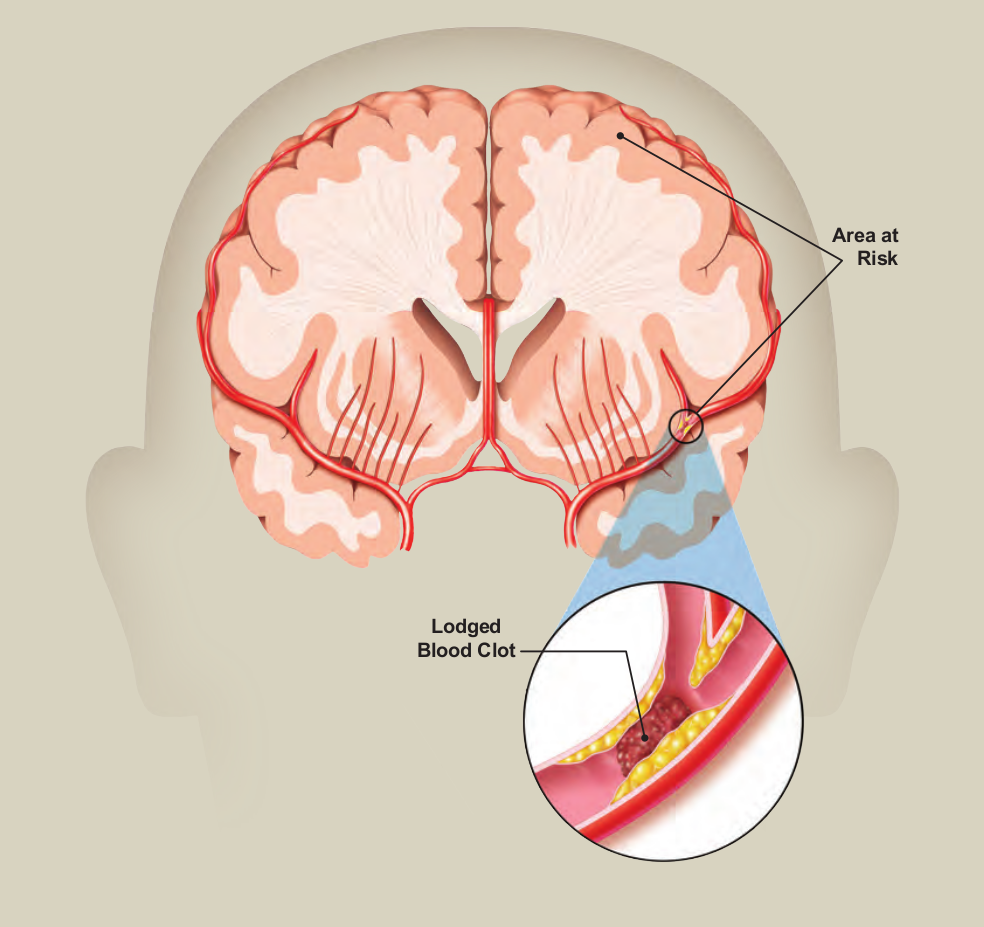
\includegraphics[height=6cm, width=5.5cm]{b6}}}
\put(200,0){\visible<2>{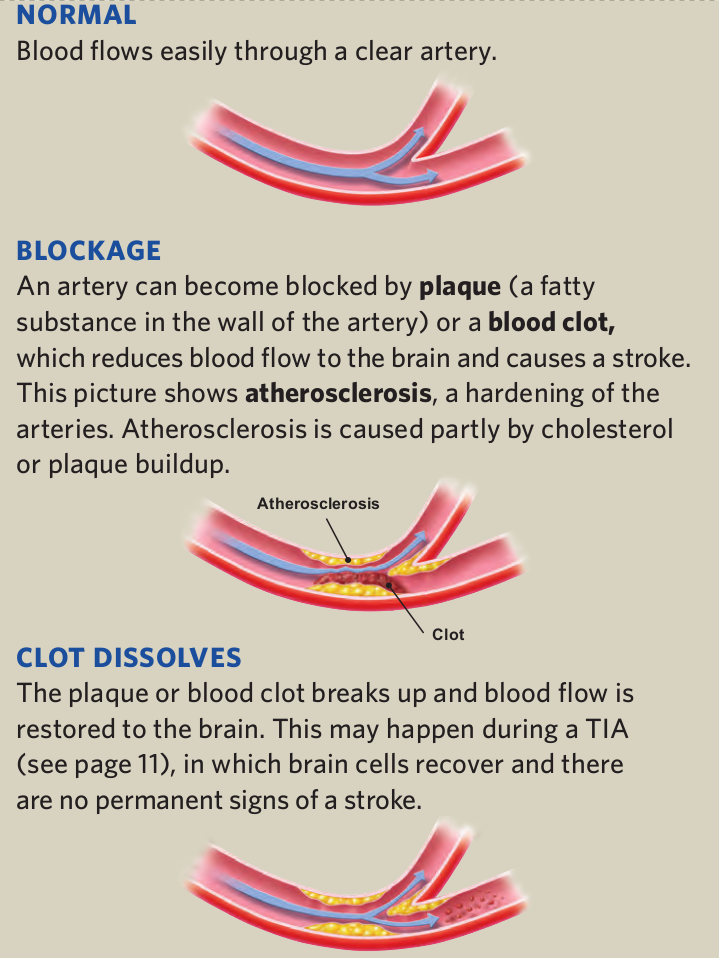
\includegraphics[height=6cm, width=4.5cm]{b3}}}
\put(0,0){\visible<4>{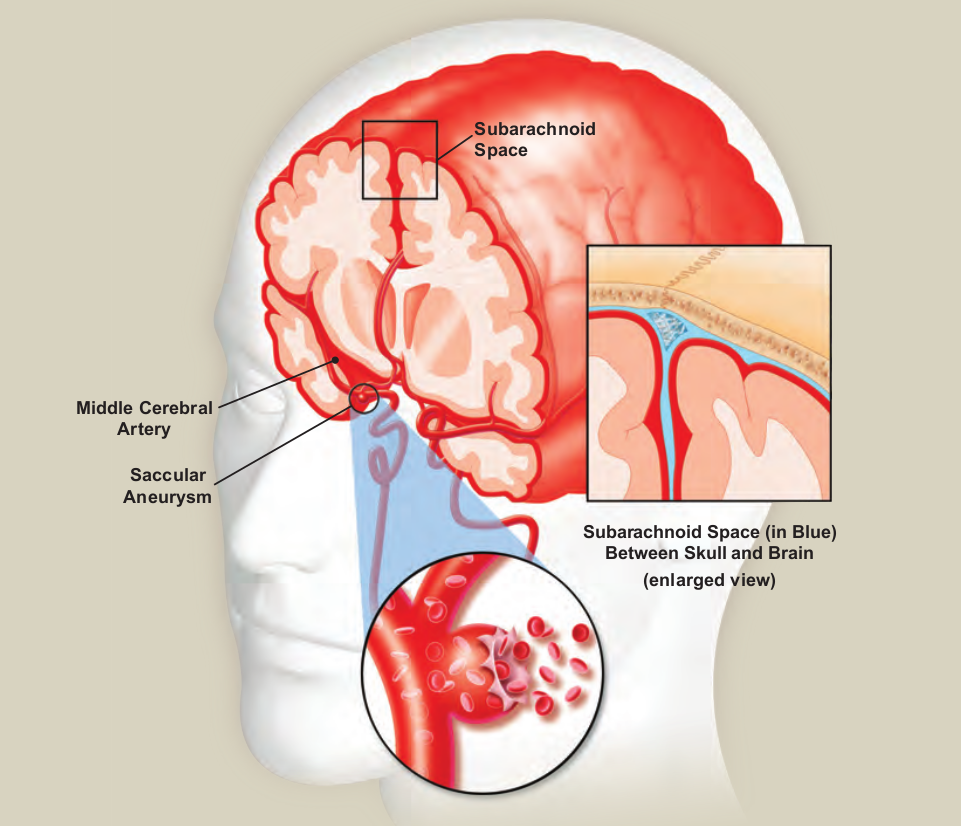
\includegraphics[height=6cm, width=6.5cm]{b4}}}
\put(172,0){\visible<4>{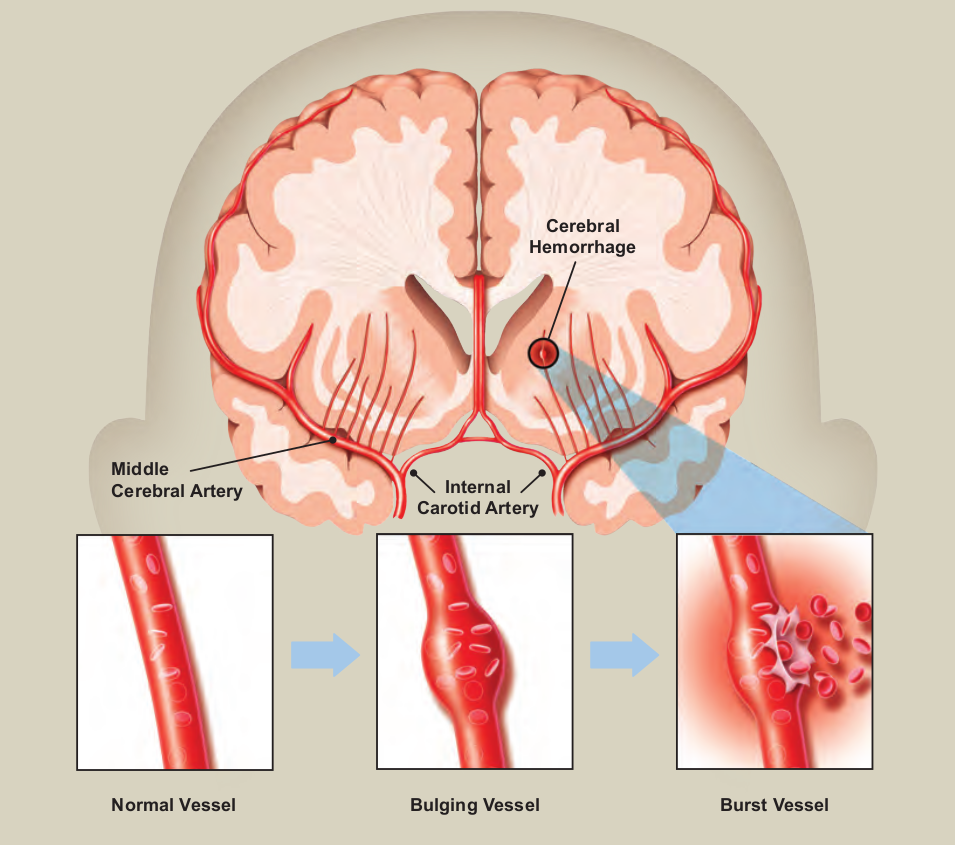
\includegraphics[height=6cm, width=6cm]{b5}}}
\end{overpic}
\end{frame}
\begin{frame}[label={sec:orgheadline4}]{Stroke therapy}
\begin{columns}
\begin{column}{0.45\columnwidth}
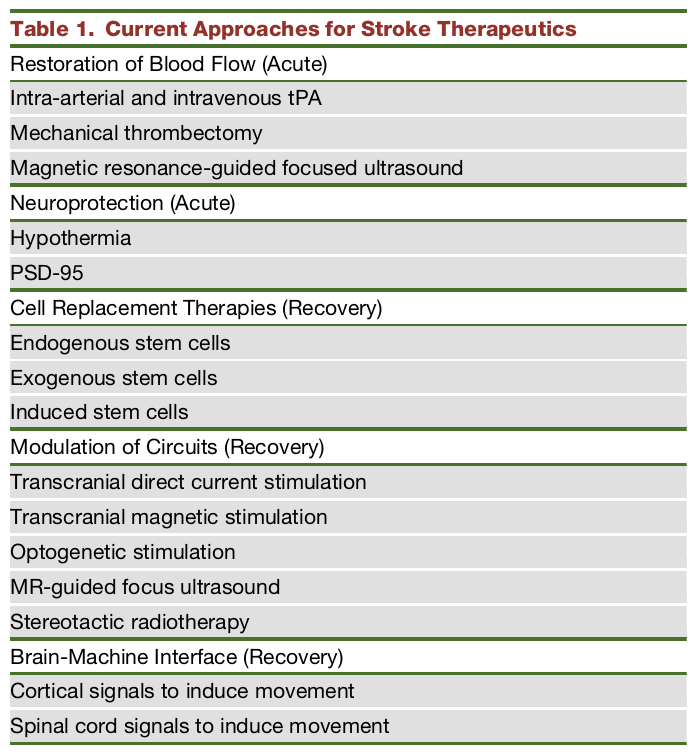
\includegraphics[height=7.6cm,width=\textwidth]{b7}
\end{column}
\begin{column}{0.55\columnwidth}
\begin{overpic}[height=6cm, width=\textwidth]{b0}
\put(0,80){\visible<2->{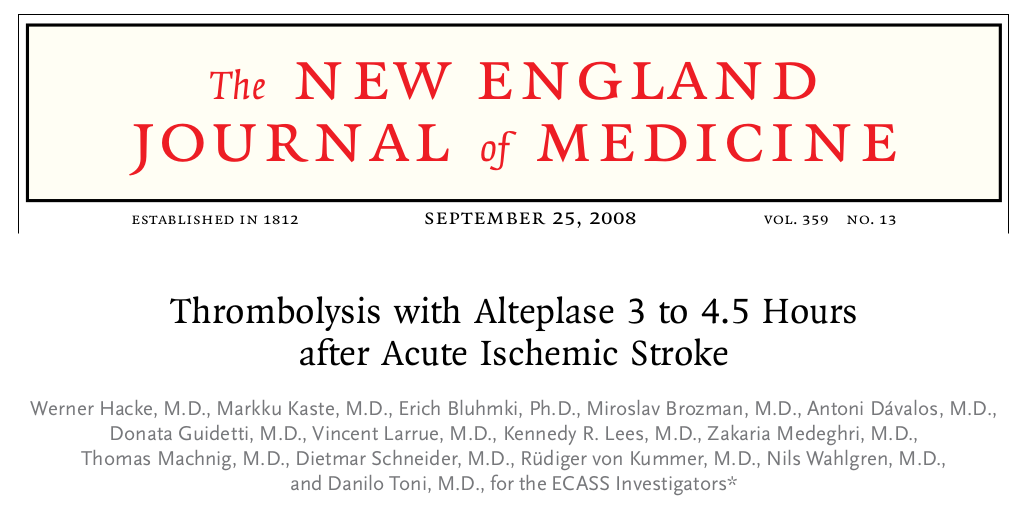
\includegraphics[height=4cm, width=\textwidth]{b11}}}
\put(0,-25){\visible<3>{
\includegraphics[height=4cm, width=\textwidth]{b12}}}
\put(0,-22){\visible<4>{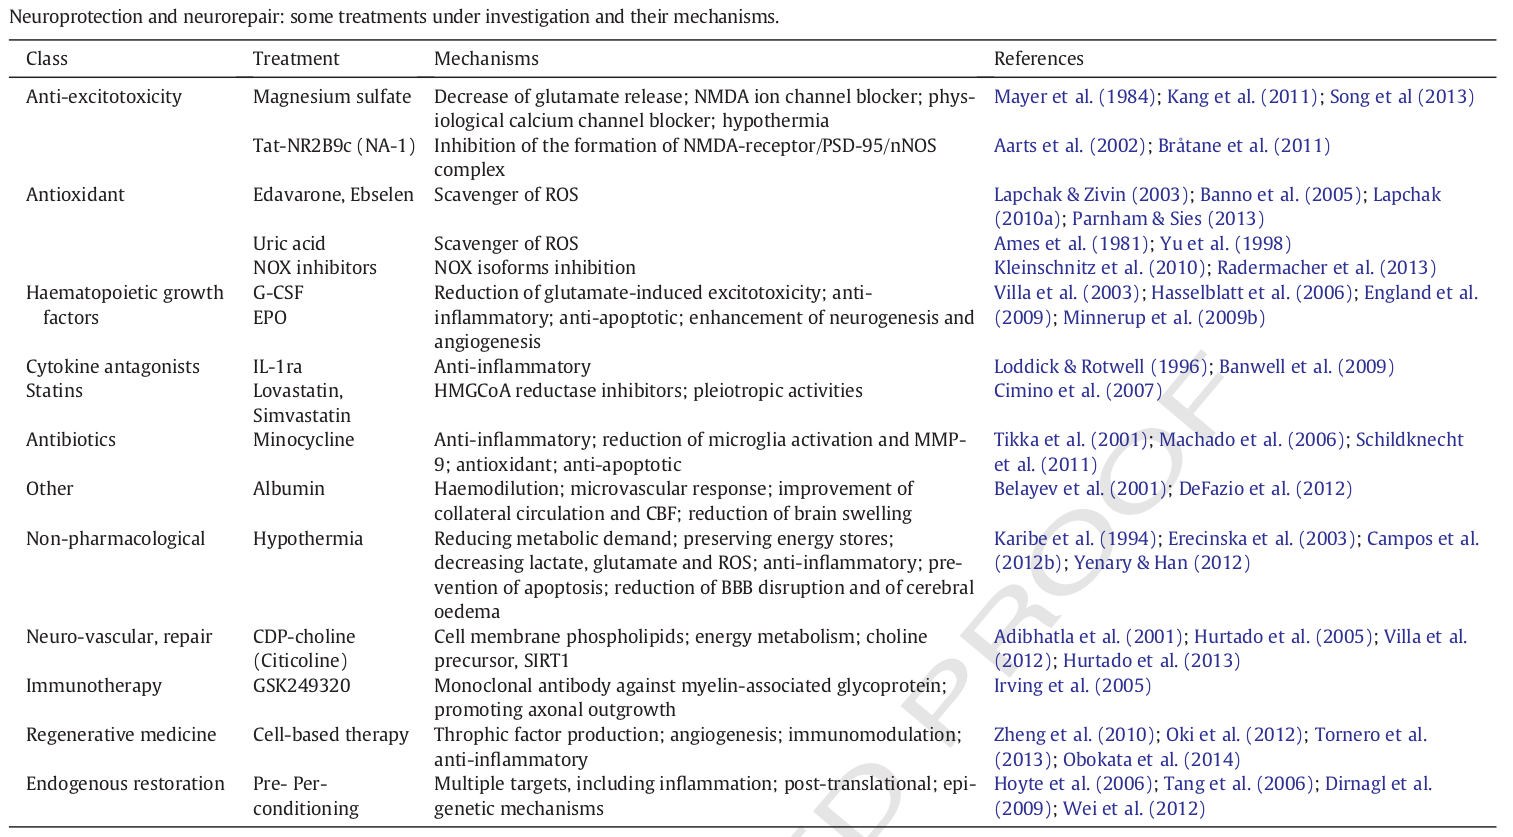
\includegraphics[height=3.6cm, width=\textwidth]{b9}}}
\end{overpic}
\end{column}
\end{columns}
\end{frame}
\begin{frame}[label={sec:orgheadline5}]{Pathophysiology of stroke}
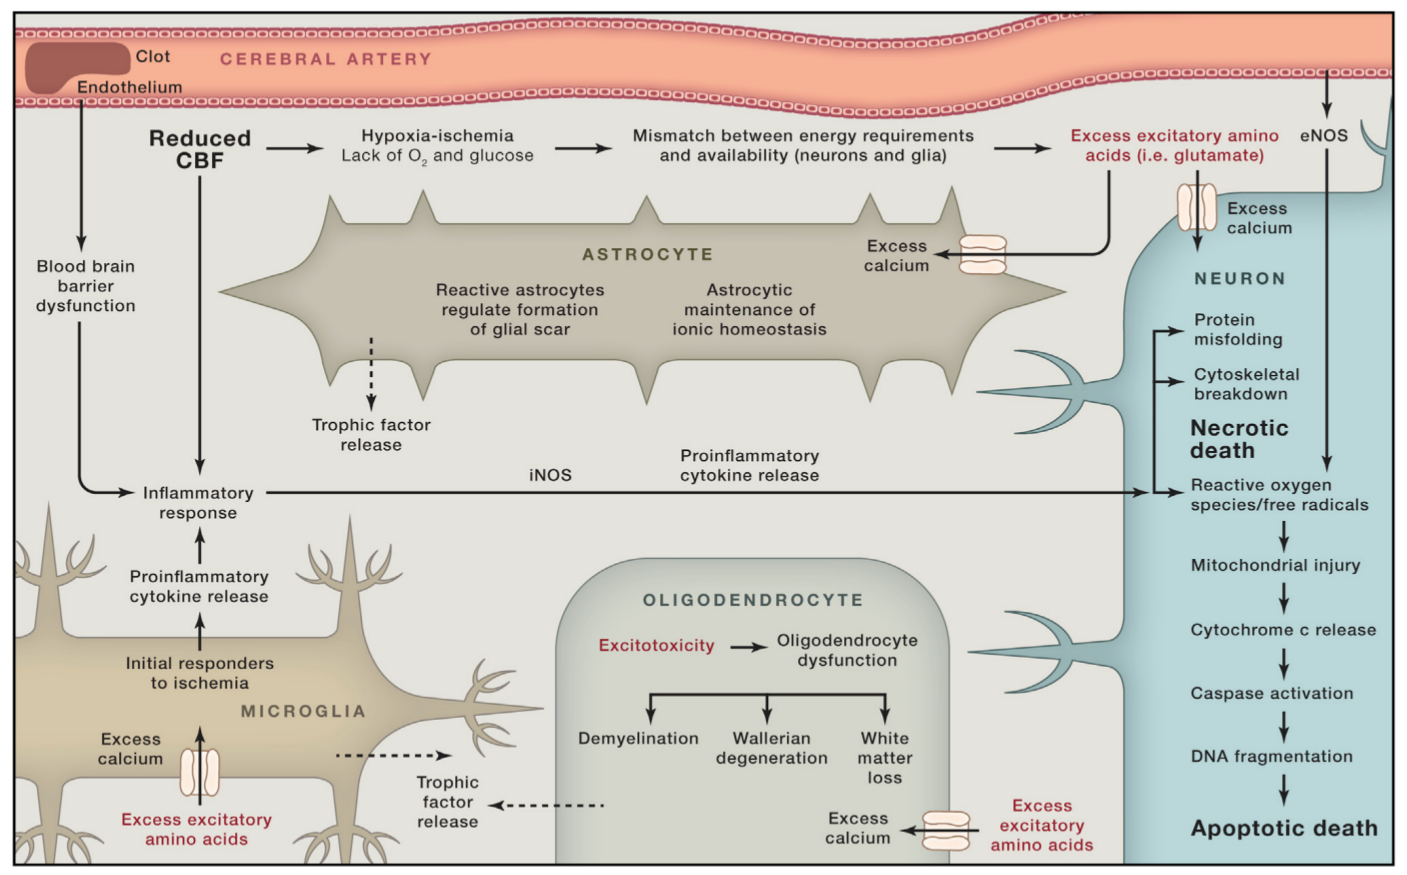
\includegraphics[height=7cm,width=\textwidth]{b8}
\end{frame}
\begin{frame}[label={sec:orgheadline6}]{Stroke therapy}
\begin{columns}
\begin{column}{0.6\columnwidth}
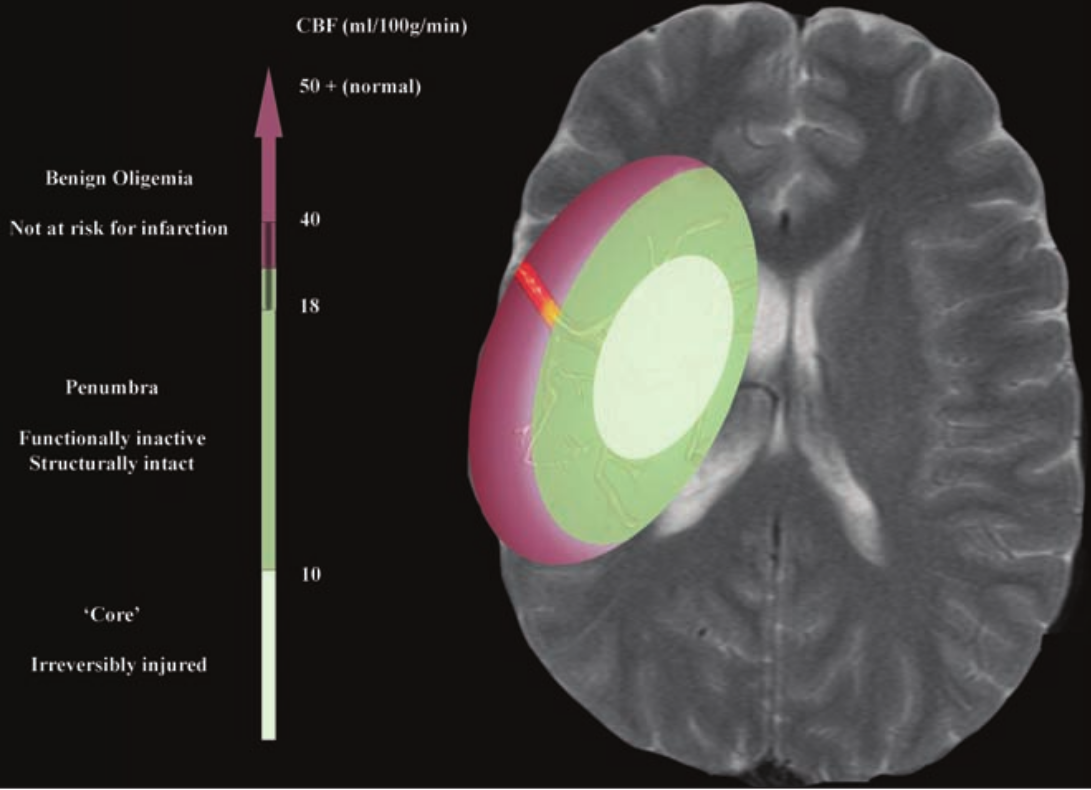
\includegraphics[height=5cm,width=\textwidth]{b10}
\end{column}
\begin{column}{0.4\columnwidth}
\begin{block}{\pause \small Stroke therapeutic strategy}
\begin{itemize}
\item \footnotesize Broaden the therapeutic time window
\begin{itemize}
 \item \scriptsize The new thrombolytics
 \item \scriptsize Neuroprotection agents-\emph{\textbf{progranulin}}
\end{itemize}
\item \footnotesize Therapy is recovery stage
\begin{itemize}
 \item \scriptsize Neuroprotection agents
 \item \scriptsize Stem cell therapy
 \item \scriptsize Chinese traditional medicine
 \item \scriptsize Acupuncture
 \item \scriptsize ......
\end{itemize}
\end{itemize}
\end{block}
\end{column}
\end{columns}
\end{frame}
\begin{frame}[label={sec:orgheadline7}]{Progranulin (PGRN)}
\begin{columns}
\begin{column}{0.8\columnwidth}
\begin{itemize}
\item A widely expressed secreted N-linked glycoprotein growth factor
\end{itemize}
\vskip 0.5cm
\begin{itemize}
\item Two isoforms:
\begin{itemize}
\item \footnotesize The glycosylated immature isoform (58–68 kDa)
\item \footnotesize The fully glycosylated mature secretory isoform (\textasciitilde{}88 kDa)
\end{itemize}
\end{itemize}
\vskip 0.5cm
\begin{itemize}
\item Mutiple physiology effects
\end{itemize}
\end{column}
\begin{column}{0.8\columnwidth}
\begin{overpic}[height=6cm, width=\textwidth]{b0}
\put(-200,0){\visible<2->{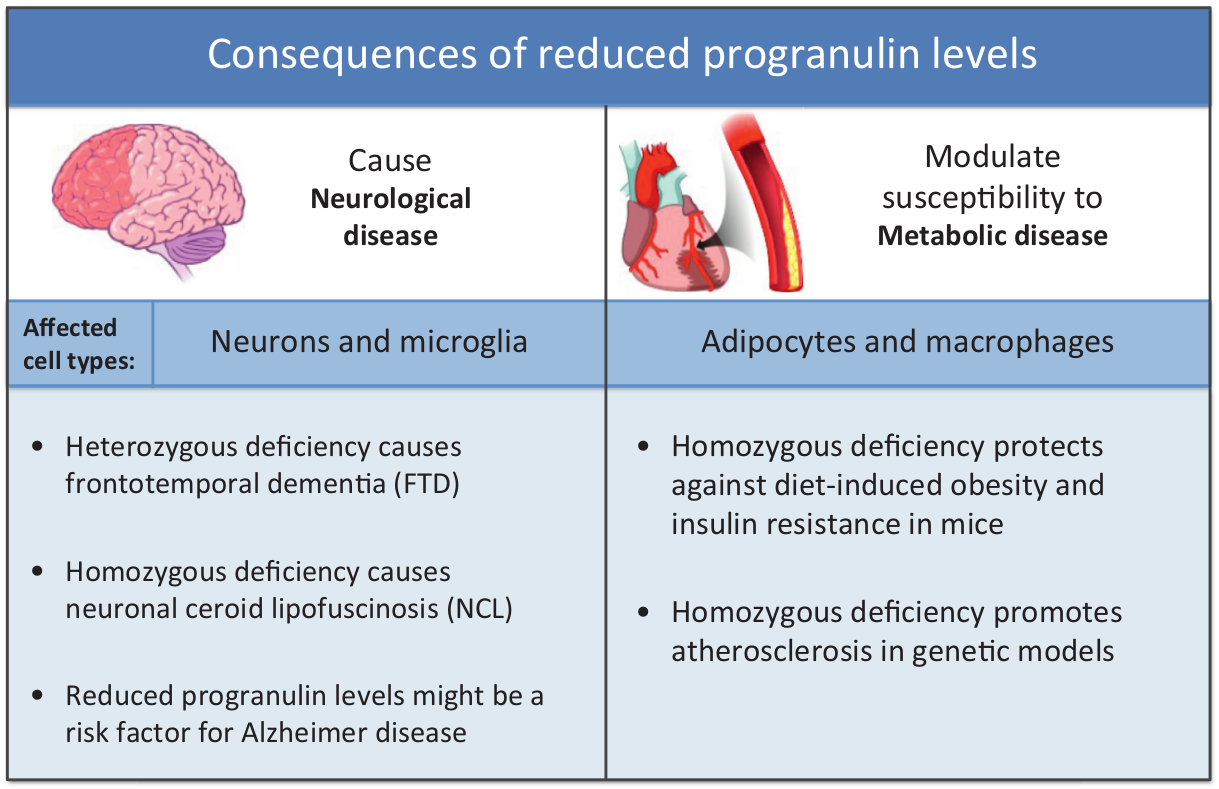
\includegraphics[height=6cm, width=\textwidth]{b13}}}
\end{overpic}
\end{column}
\end{columns}
\end{frame}
\begin{frame}[label={sec:orgheadline8}]{The relationship of PGRN and stroke}
\begin{block}{First, Protecd vascular from cerebral ishcemia}
\begin{itemize}
\item \footnotesize Recombinant PGRN could suppress cerebral oedema in focal MCAO
\item \footnotesize PGRN knockout mice prompt post-ischaemic BBB disruption
\end{itemize}
\end{block}
\begin{block}{\pause Second, PGRN is involved in neuroinflammation}
\begin{itemize}
\item \footnotesize PGRN was induced in activated microglia
\item \footnotesize Microglia activation incresed infract area in ischemia
\item \footnotesize PGRN suppress secretion of pro-inflammatory cytokines and recruitment of neutrophils
\end{itemize}
\end{block}
\begin{block}{\pause Third, PGRN exhibit protective effects on neuronal cells}
\begin{itemize}
\item \footnotesize TARDBP (TDP-43) is involved in cerebral ischemia
\item \footnotesize PGRN inhibite caspase 3 to suppress TARDBP cleavage
\end{itemize}
\end{block}
\end{frame}
\begin{frame}[label={sec:orgheadline9}]{Aim to study}
\begin{block}{The study were designed to clarify the effetcts of PGRN on regulation of blood–brain barrier function, suppression of inflammation, and neuroprotection against acute focal cerebral ischaemia.}
\end{block}
\end{frame}
\section{Materials and Methods}
\label{sec:orgheadline14}
\begin{frame}[label={sec:orgheadline11}]{Methods used in the article}
\begin{block}{Focal cerebral ischaemia model}
\end{block}
\begin{block}{Immunoblotting}
\end{block}
\begin{block}{Immunofluorescence staining and confocal microscopy}
\end{block}
\begin{block}{Immunohistochemistry}
\end{block}
\begin{block}{Measurement of the volume of the cerebral infarct and oedema}
\end{block}
\begin{block}{Neurological evaluations}
\end{block}
\end{frame}
\begin{frame}[label={sec:orgheadline12}]{Methods used in the article}
\begin{block}{C6 cell culture and analysis of glycosylation}
\end{block}
\begin{block}{Primary cell cultures}
\end{block}
\begin{block}{Oxygen–glucose deprivation}
\end{block}
\begin{block}{Cell counting protocols}
\end{block}
\begin{block}{PCR and quantitative real-time PCR}
\end{block}
\begin{block}{Focal embolic ischaemia model}
\end{block}
\end{frame}
\begin{frame}[label={sec:orgheadline13}]{Markers used in the article}
\begin{columns}
\begin{column}{0.6\columnwidth}
\begin{itemize}
\item MAP2-neuronal cells
\item ERp57-endoplasmic reticulum
\item Golgi-58k-Golgi apparatus
\item LAMP1-lysosome
\item CD68/ED1-microglia
\item DAPI-neuclei
\item vWF,CD31-endothelial cells
\item GFAP-astrocytes
\end{itemize}
\end{column}
\begin{column}{0.5\columnwidth}
\begin{overpic}[height=6cm, width=12cm]{b0}
\put(0,0){\visible<2->{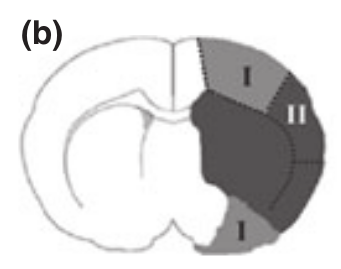
\includegraphics[height=4cm, width=5cm]{m1}}}
\end{overpic}
\end{column}
\end{columns}
\end{frame}
\section{Results}
\label{sec:orgheadline24}
\begin{frame}[label={sec:orgheadline15}]{\small The expression and localization of PGRN on non-ischemia cortex}
\begin{overpic}[height=6cm, width=12cm]{b0}
\put(-7,-10){\visible<1->{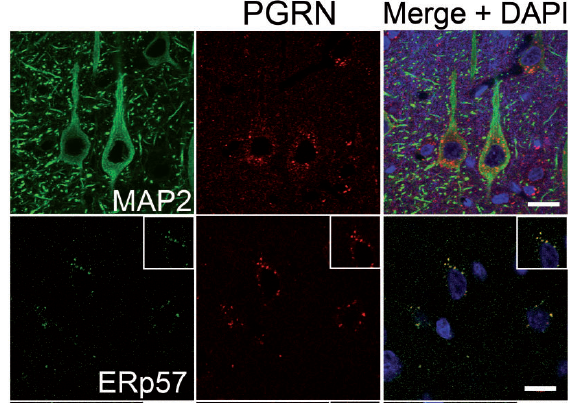
\includegraphics[height=5cm, width=6.2cm]{f11}}}
\put(170,-10){\visible<2>{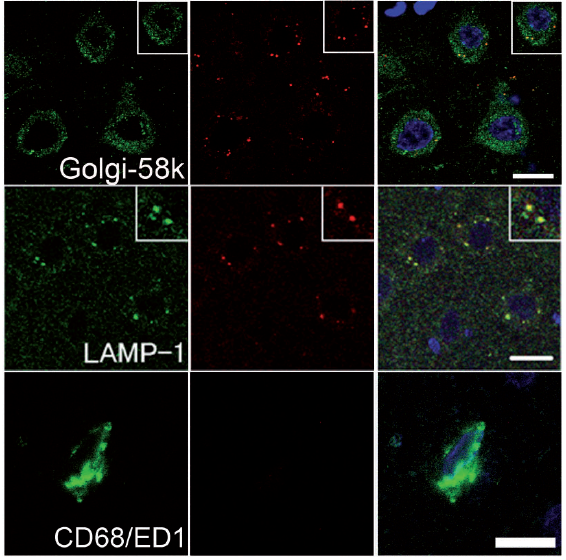
\includegraphics[height=6cm, width=6.2cm]{f12}}}
\end{overpic}
\vskip 0.5cm \scriptsize MAP2-neuronal cells ERp57-endoplasmic reticulum Golgi-58k-Golgi apparatus LAMP1-lysosome CD68/ED1-microgliay
\end{frame}
\begin{frame}[label={sec:orgheadline16}]{\small The expression and localization of PGRN on ischemia cortex}
\begin{overpic}[height=6cm, width=12cm]{b0}
\put(-7,70){\visible<1->{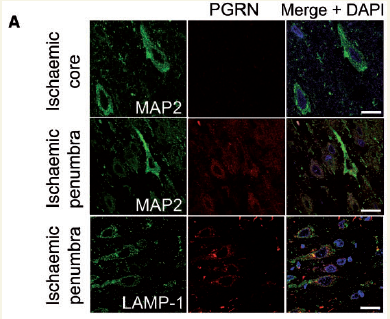
\includegraphics[height=3.5cm, width=6.2cm]{f21}}}
\put(-7,-30){\visible<2->{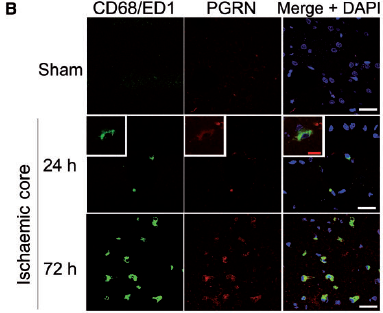
\includegraphics[height=3.5cm, width=6.2cm]{f22}}}
\put(171,-30){\visible<3>{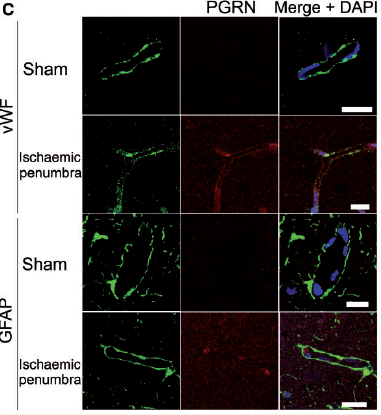
\includegraphics[height=7cm, width=6.2cm]{f23}}}
\end{overpic}
\vskip 1.2cm \scriptsize vWF-endothelial cells GFAP-astrocytes
\end{frame}
\begin{frame}[label={sec:orgheadline17}]{\small PGRN temporal changes and its glycosylated status after ischemia}
\begin{overpic}[height=6cm, width=12cm]{b0}
\put(0,-20){\visible<1>{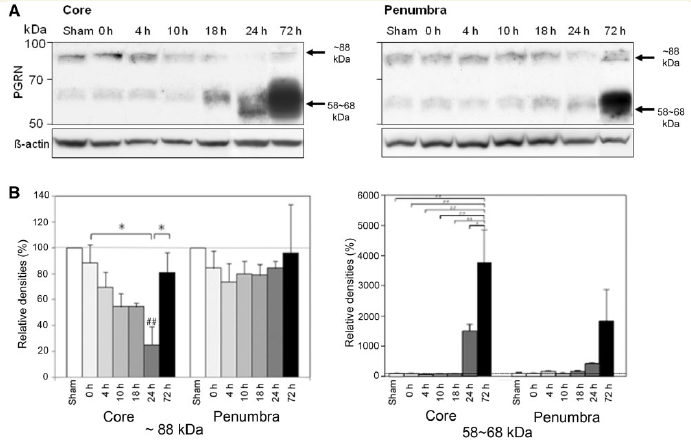
\includegraphics[height=7cm, width=12cm]{f31}}}
\put(80,10){\visible<2>{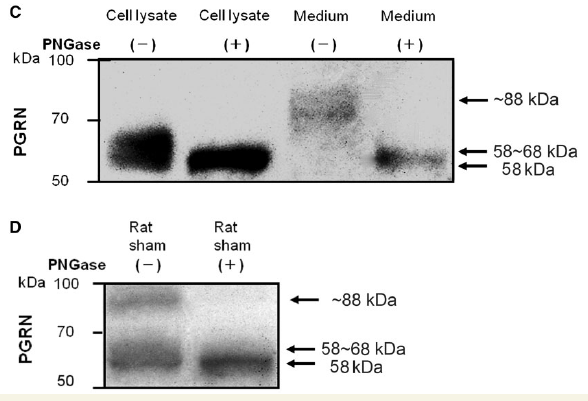
\includegraphics[height=5cm, width=7cm]{f32}}}
\end{overpic}
\end{frame}
\begin{frame}[label={sec:orgheadline18}]{\small Production and secretion of the two isoforms of PGRN after OGD}
\begin{overpic}[height=6cm, width=12cm]{b0}
\put(-7,20){\visible<1->{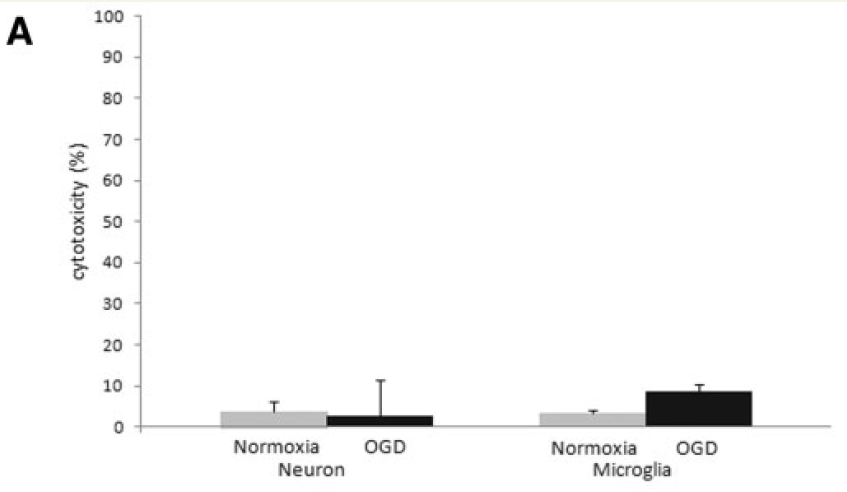
\includegraphics[height=3.8cm, width=6.2cm]{f41}}}
\put(171,76){\visible<2->{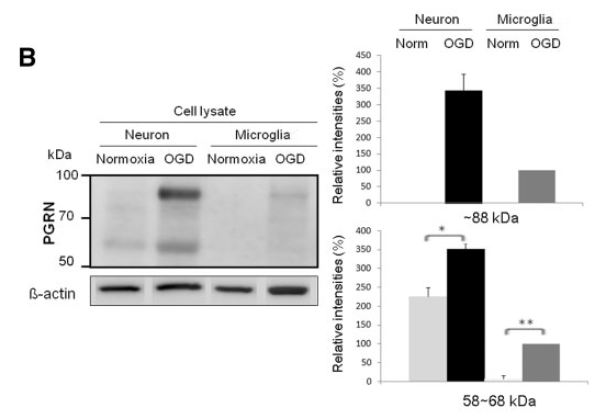
\includegraphics[height=3.8cm, width=6.2cm]{f42}}}
\put(171,-30){\visible<2->{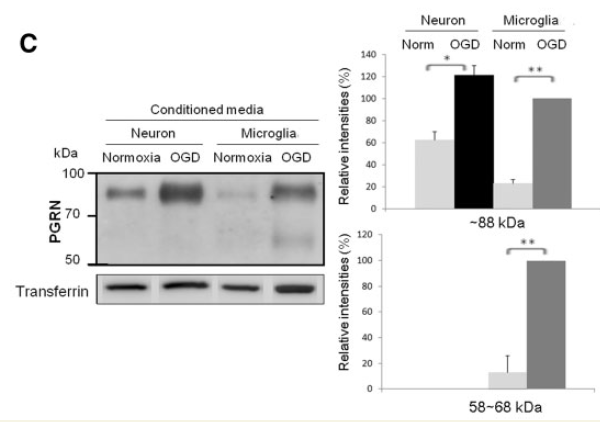
\includegraphics[height=3.8cm, width=6.2cm]{f43}}}
\end{overpic}
\end{frame}
\begin{frame}[label={sec:orgheadline19}]{Summary}
\begin{itemize}
\item The author demonstrated a dynamic change in progranulin expression:
\begin{itemize}
\item \footnotesize PGRN's expression in microglia increased in the border of ischemic core and penumbra
\item \footnotesize PGRN's expression in viable neurons increased within the ischemic penumbra
\item \footnotesize PGRN's expression in endothelial cells increased within ischemia penumbra
\end{itemize}
\item \textasciitilde{}88 kDa progranulin decreased, whereas the 58–68 kDa progranulin markedly increased at 24 h and 72 h after reperfusion
\item 58-68 kDa PGRN was secreted only from the microglia after ischemia
\end{itemize}
\end{frame}
\begin{frame}[label={sec:orgheadline20}]{\small PGRN attenuate BBB disruption after cerebral ischaemia via VEGF}
\begin{overpic}[height=6cm, width=12cm]{b0}
\put(0,-20){\visible<1>{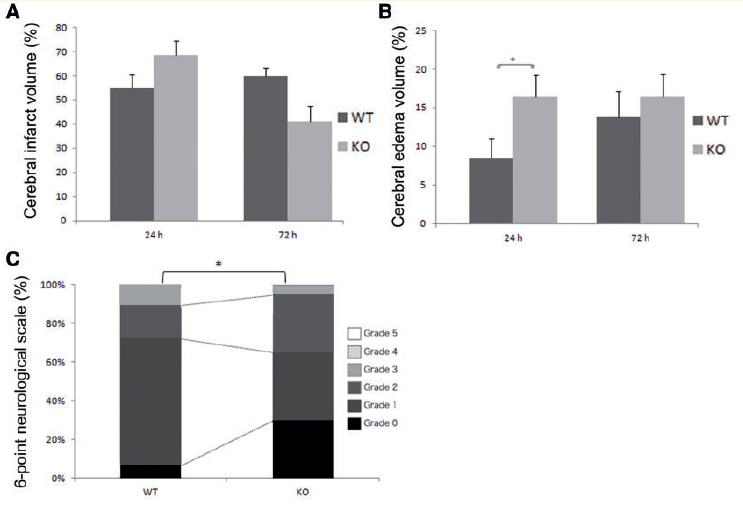
\includegraphics[height=7cm, width=12cm]{f51}}}
\put(40,-20){\visible<2>{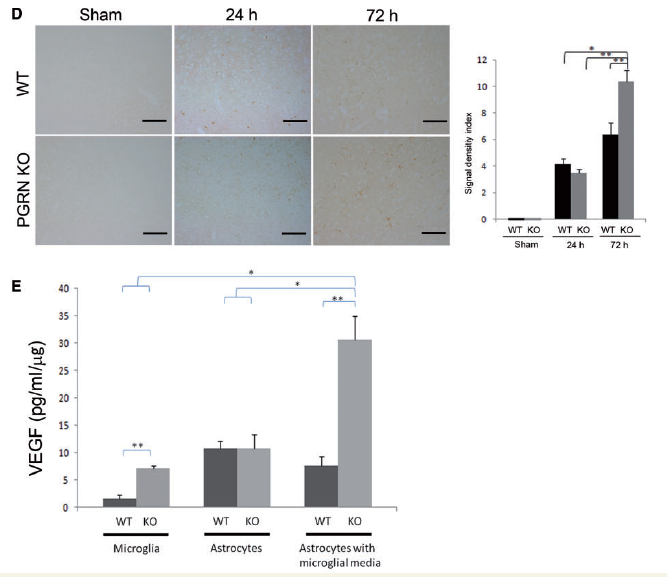
\includegraphics[height=7cm, width=10cm]{f52}}}
\end{overpic}
\end{frame}
\begin{frame}[label={sec:orgheadline21}]{\small PGRN suppress neuroinflammation after cerebral ishcemia via IL-10}
\begin{overpic}[height=6cm, width=12cm]{b0}
\put(-7,76){\visible<1->{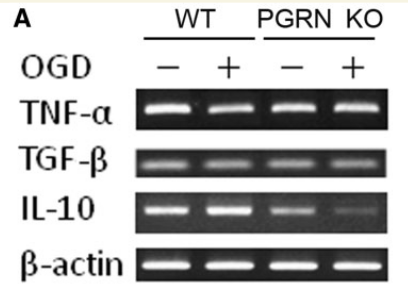
\includegraphics[height=3.8cm, width=6.2cm]{f61}}}
\put(0,-30){\visible<1->{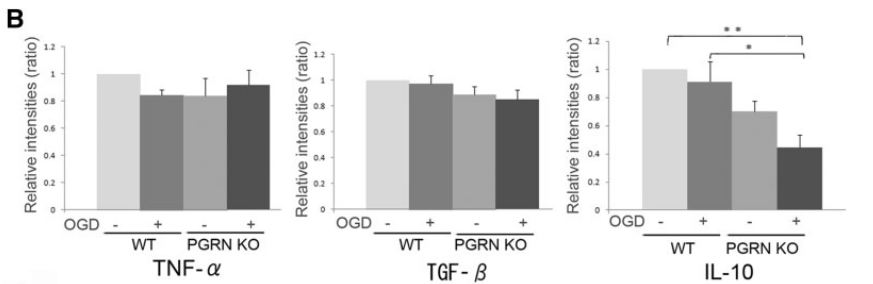
\includegraphics[height=3.8cm, width=12cm]{f62}}}
\put(170,76){\visible<2->{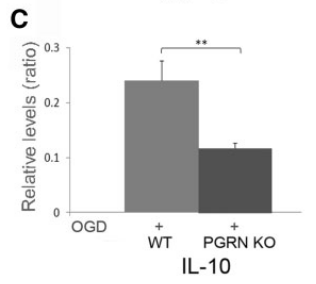
\includegraphics[height=3.8cm, width=6.2cm]{f63}}}
\end{overpic}
\end{frame}
\begin{frame}[label={sec:orgheadline22}]{\small PGRN protect neuron from cerebral ischemia in part by the inhibition of abnormal cytoplasmic redistribution of nuclear TARDBP}
\begin{overpic}[height=6cm, width=12cm]{b0}
\put(0,-10){\visible<1>{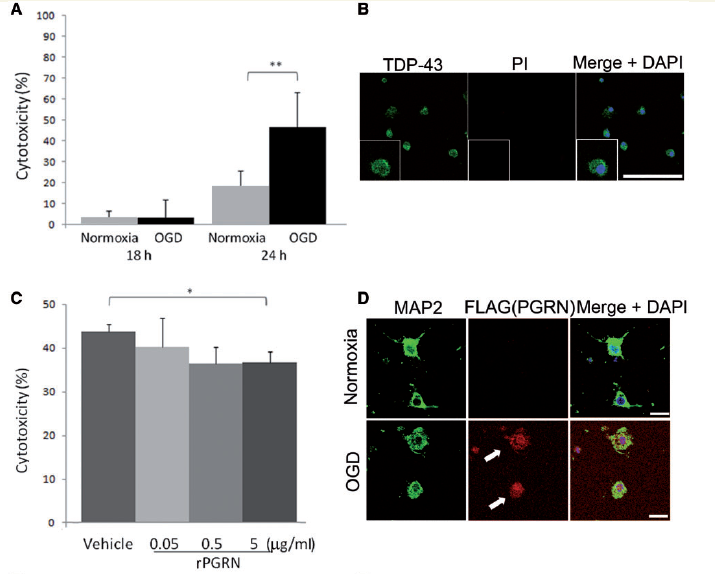
\includegraphics[height=6.5cm, width=12cm]{f71}}}
\put(0,0){\visible<2>{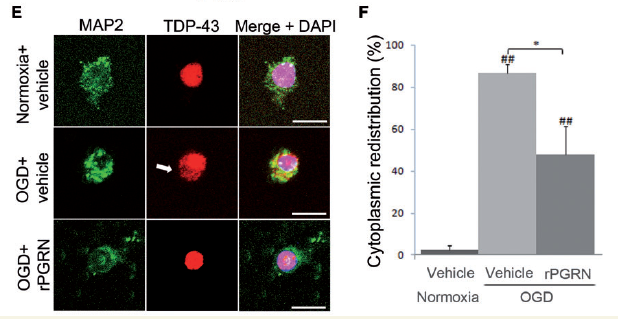
\includegraphics[height=6cm, width=12cm]{f72}}}
\end{overpic}
\end{frame}
\begin{frame}[label={sec:orgheadline23}]{\small Therapeutic effects of PGRN with tPA for cerebral ischaemia}
\begin{overpic}[height=6cm, width=12cm]{b0}
\put(40,-20){\visible<1>{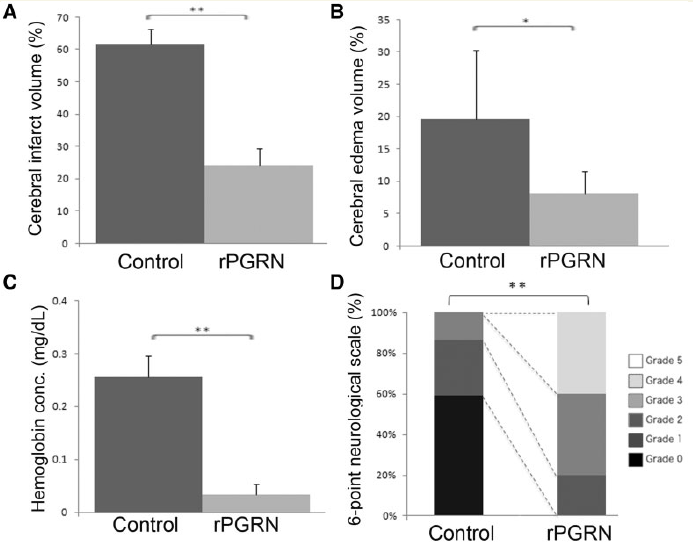
\includegraphics[height=7cm, width=10cm]{f81}}}
\put(40,-20){\visible<2>{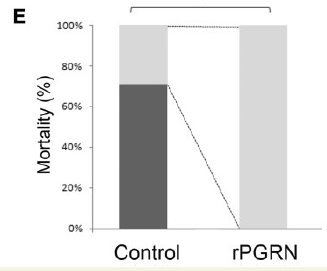
\includegraphics[height=6cm, width=10cm]{f82}}}
\end{overpic}
\end{frame}

\section{Conclusion}
\label{sec:orgheadline31}
\begin{frame}[label={sec:orgheadline25}]{Conculsion}
\begin{itemize}
\item First, the author firstly demonstrated the dynamic changes of PGRN, and the 58-68 kDa PGRN was secreted only from the microglia after ischemia
\end{itemize}
\vskip 0.5cm
\begin{itemize}
\item Sceond, PGRN provides vascular protection, anti-neuroinflammation, and neuroprotection related in part to VEGF, IL10 and TARDBP
\end{itemize}
\vskip 0.5cm
\begin{itemize}
\item Third, the possibility that recombinant PGRN could be used as a novel neurovascular protective drug with anti-inflammatory effect after delayed tPA treatment
\end{itemize}
\end{frame}
\begin{frame}[label={sec:orgheadline26}]{References}
\tiny
\cite{moretti2015neuroprotection} \cite{george2015novel} \cite{butcher2010acute} \cite{hacke2008thrombolysis} \cite{kanazawa2011biochemical} \cite{kanazawa2011inhibition} \cite{nguyen2013progranulin} \cite{o20061}
\printbibliography[heading = none]
\end{frame}
\begin{frame}[label={sec:orgheadline27}]{Some Comments of mine}
\begin{block}{The study design is complete}
\end{block}
\begin{block}{\pause But}
\begin{itemize}
\item The precise mechnisms of PGRN on ischemia
\item \pause Wentern blot results isn't beautiful
\item \pause The MCAO model validation standard
\end{itemize}
\end{block}
\end{frame}
\begin{frame}[label={sec:orgheadline28}]{Focal cerebral ischemia model}
\begin{columns}
\begin{column}{0.5\columnwidth}
\vskip 3.5cm
\hskip 0.2cm \small Focal ischemia model validation \\ \hskip 0.2cm standard
\begin{itemize}
\item \footnotesize I -30 min CBF Baseline 100\%
\item \footnotesize I 10 min CBF < 20\% , \newline I 80 min CBF < 20\%
\item \footnotesize R 10 min CBF > 70\%
\end{itemize}
\end{column}
\begin{column}{1.0\columnwidth}
\begin{overpic}[height=6cm, width=\textwidth]{b0}
\put(-165,-20){\visible<1>{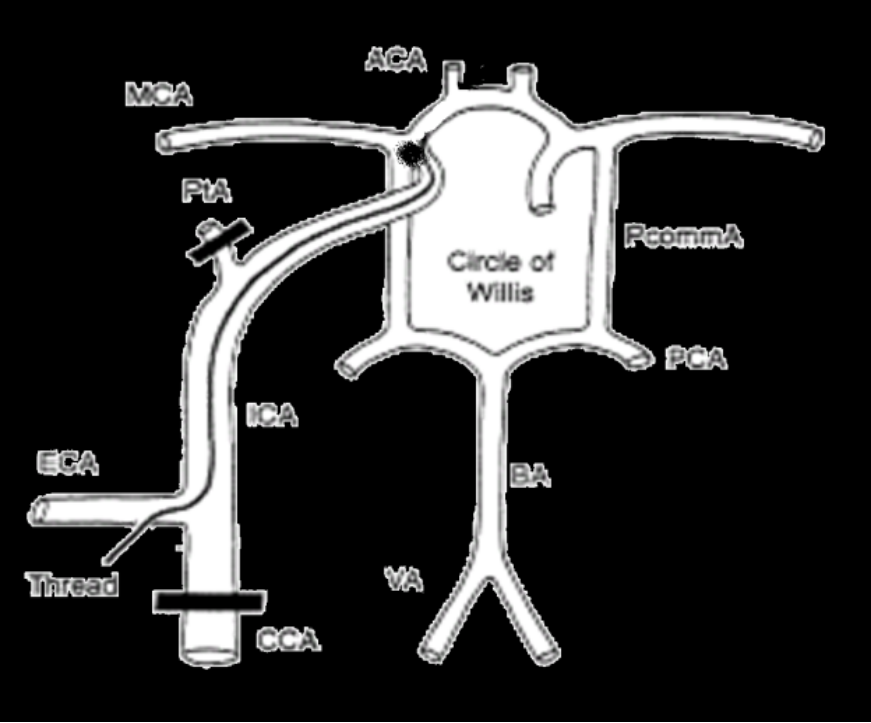
\includegraphics[height=7cm, width=0.65\textwidth]{b16}}}
\put(-160,100){\visible<2->{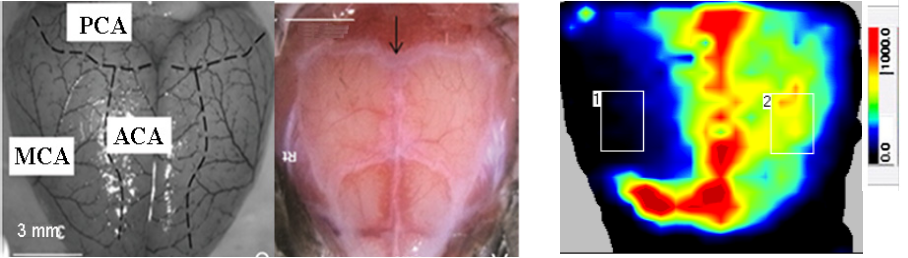
\includegraphics[height=3cm, width=\textwidth]{b14}}}
\put(20,-25){\visible<2->{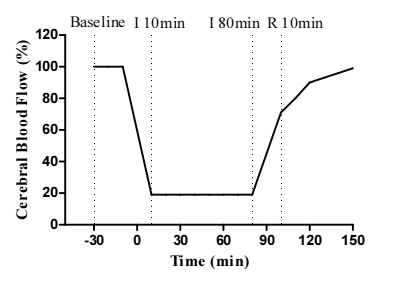
\includegraphics[height=4cm, width=0.5\textwidth]{b15}}}
\end{overpic}
\end{column}
\end{columns}
\end{frame}
\begin{frame}[label={sec:orgheadline29}]{Methods to search and obtain the article}
\begin{overpic}[height=6cm, width=12cm]{b0}
\put(0,-20){\visible<1>{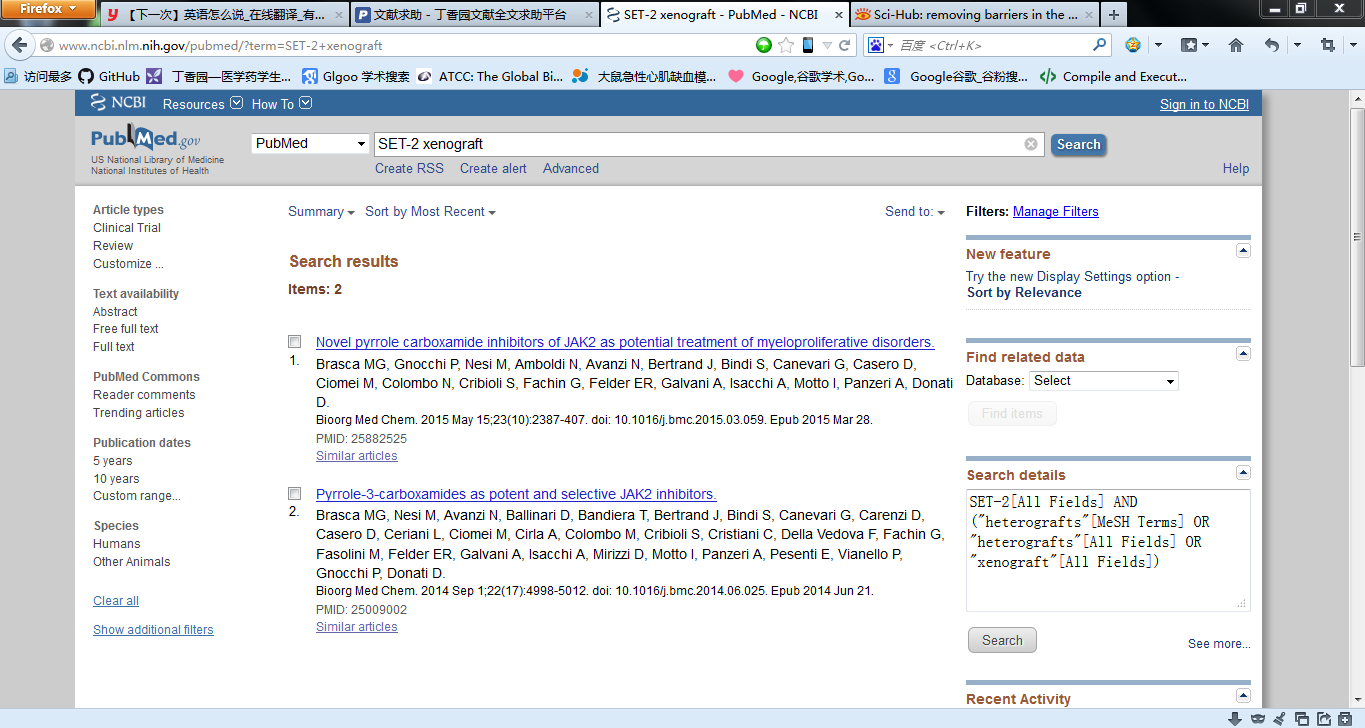
\includegraphics[height=7cm, width=12cm]{1-1}}}
\put(0,-20){\visible<2>{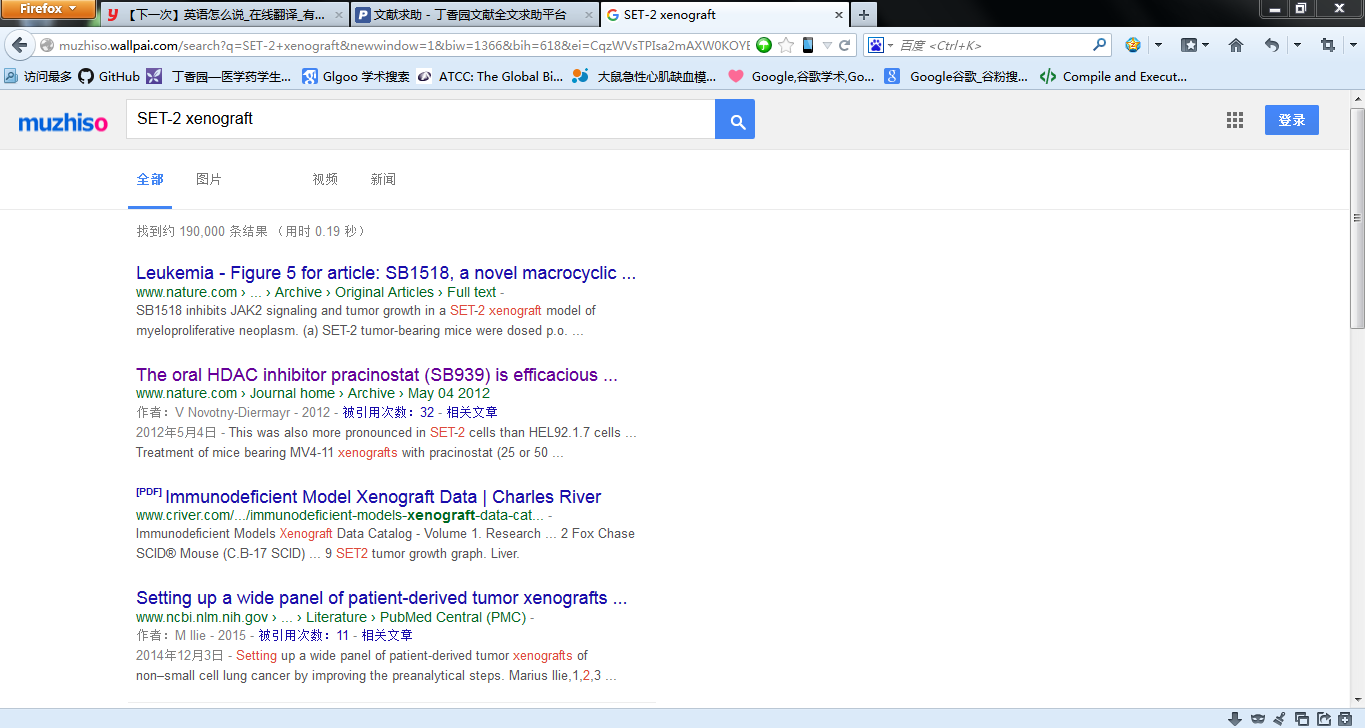
\includegraphics[height=7cm, width=12cm]{1-2}}}
\put(0,-20){\visible<3>{
\includegraphics[height=7cm, width=12cm]{2-1}}}
\put(0,-20){\visible<4>{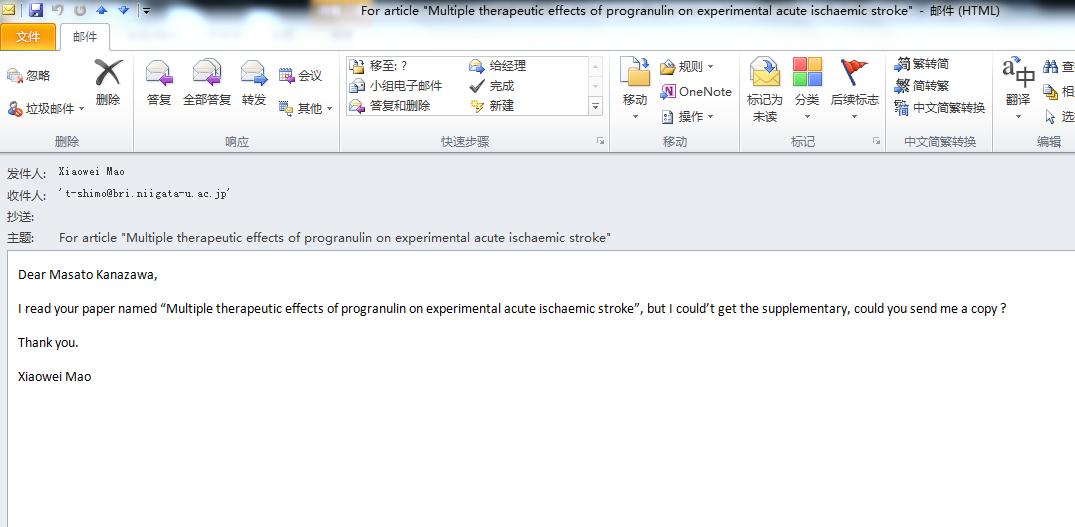
\includegraphics[height=7cm, width=12cm]{2-2}}}
\put(0,-20){\visible<5>{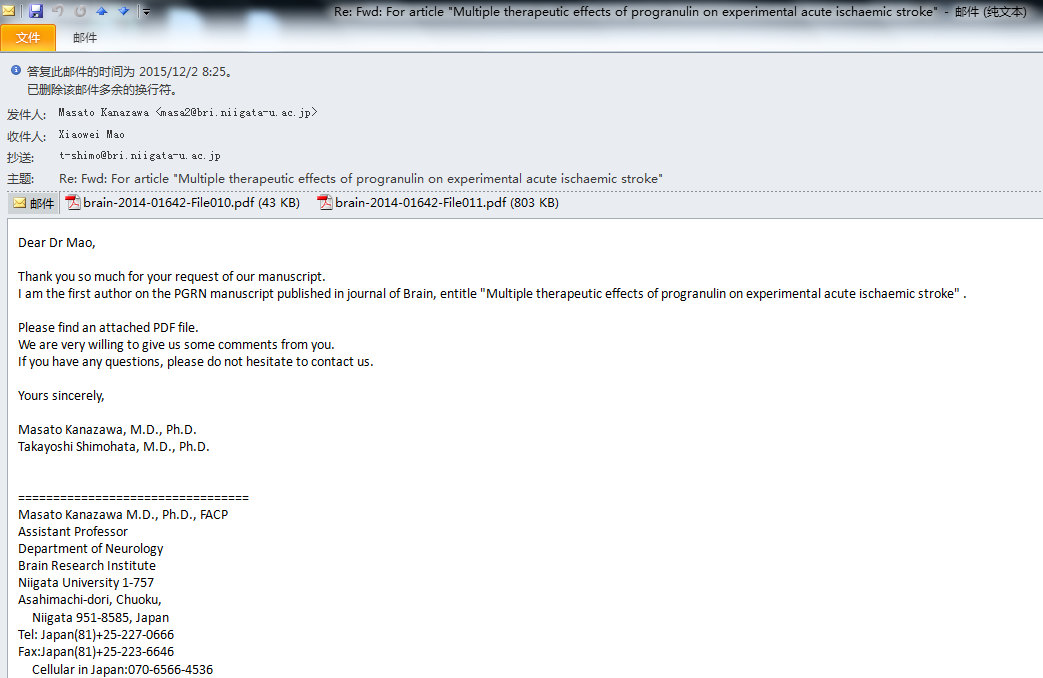
\includegraphics[height=7cm, width=12cm]{2-3}}}
\put(0,-20){\visible<6>{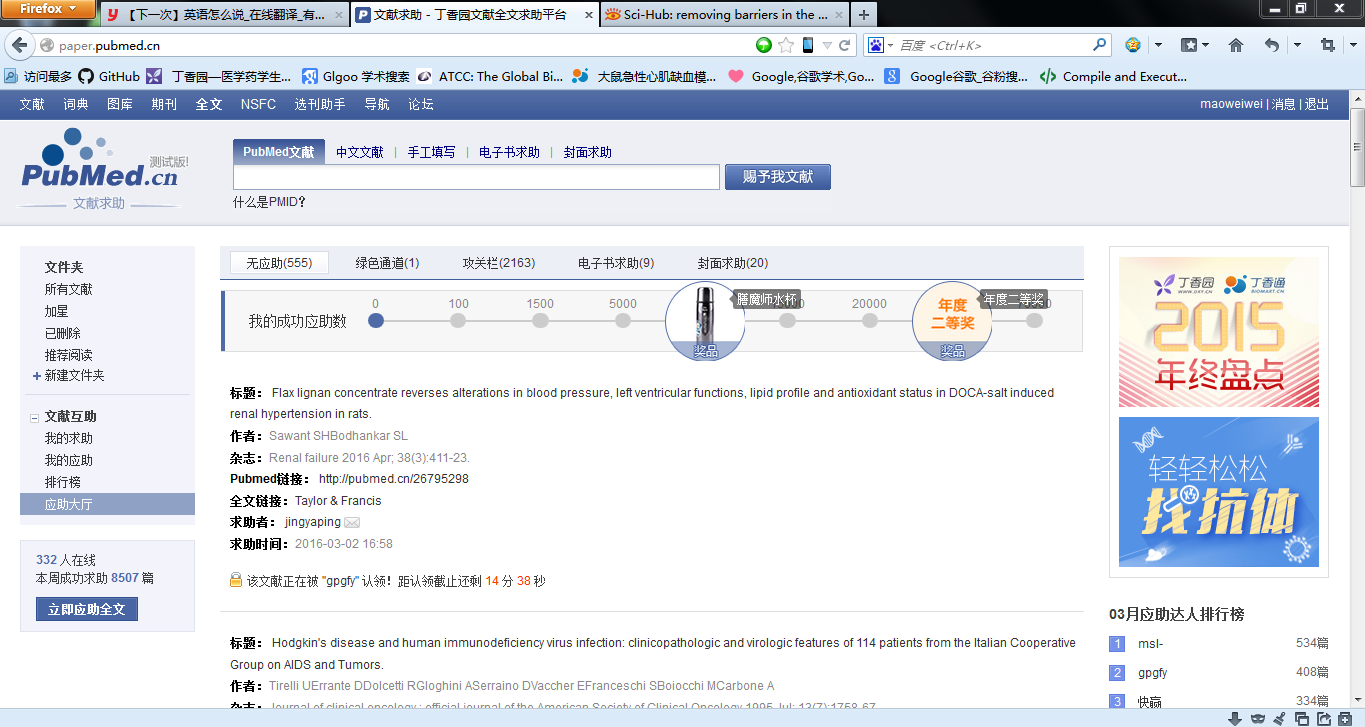
\includegraphics[height=7cm, width=12cm]{2-4}}}
\end{overpic}
\end{frame}
\begin{frame}[label={sec:orgheadline30}]{}
\huge Thanks for your attention.
\vskip 3cm
\centering \Huge Questions?
\end{frame}
\end{document}